%\documentclass[a4paper,12pt]{report}
\documentclass[finnish,12pt]{article}
%\usepackage[utf8]{inputenc}
\usepackage[utf8]{inputenc}
\usepackage[finnish]{babel}
\usepackage{ae,aecompl}

\usepackage[pdftex]{graphicx}
\usepackage{url}
%% Matematiikan fontteja, symboleja ja muotoiluja
\usepackage{amsfonts,amssymb,amsbsy}
%% Taulukon paketti
%\usepackage{multirow}

%% Vaakasuunnan mitat, EI KOSKE!
\setlength{\hoffset}{-1in}
\setlength{\oddsidemargin}{35mm}
\setlength{\evensidemargin}{20mm}
\setlength{\textwidth}{15cm}
%% Pystysuunnan mitat, EI KOSKE!
\setlength{\voffset}{-1.5in}
%\setlength{\headsep}{7mm}
%\setlength{\headheight}{1em}
\setlength{\topmargin}{25mm}
\setlength{\textheight}{24cm}
%% Vasensuora-asettelu, joka opinnaytteessa vaaditaan. aLa KOSKE
\setlength{\parindent}{0pt}
\setlength{\parskip}{1ex}

%% bibtex-tyyli
\bibliographystyle{unsrt_fin}

% Title Page
\title{AS-0.3200 Automaatio- ja systeemitekniikan projektityöt: S11-15 LED-monimuuttujasäätö}
\author{Mikko Tuohimaa}
\date{13.5.2011}


\begin{document}
\maketitle
\pagenumbering{roman}
\setcounter{page}{1}
%\begin{abstract}
%\end{abstract}

%\clearpage
\tableofcontents
\clearpage

% Aloitetaan arabialainen numerointi vasta tasta
\pagenumbering{arabic}
\setcounter{page}{1}

\section{Johdanto}

Pintaverisuonia voidaan kuvata indosyaniinivihreän (ICG) avulla, joka on suurikokoinen orgaaninen molekyyli. Se sitoutuu tiukasti veriplasman proteiineihin ja sillä on erikoiset optiset ominaisuudet: sen absorptiomaksimi on 800 nanometrin kohdalla ja emissiomaksimi puolestaan 835 nm:n kohdalla, joten valaisemalla ihoa pienemmällä aallonpituudella ja kuvaamalla sitä alipäästöfiltterin läpi, nähdään vain ICG:n tuottama toisioemissio. Koska molekyyli sitoutuu vereen, saadaan näin näkyviin verisuonisto varsin vähällä invaasiolla. Infrapunavalo tunkeutuu kudokseen ainakin muutaman senttimetrin syvyydelle, joten kuvaaminen ei rajoitu pinnan hiussuoniin. \cite{Owens} \cite{Wikipedia}

ICG:n puoliintumisaika elimistössä on potilaasta riippuen 150-180 sekuntia \cite{Owens}, mikä asettaa haasteita jatkuvalle kuvaamiselle esim. intravaskulaaristen operaatioiden aikana. Tässä työssä kehitettiin automaattisesti säätyvä IR-LED-valaisin, joka adaptoituu ICG:n vasteeseen ajan funktiona tuottaen mahdollisimman selkeän kuvan.

\section{Systeemin kuvaus}

\subsection{Arkkitehtuuri}

Kuvassa \ref{fig:kommunikaatio} on esitetty systeemin kommunikaatio\-arkkitehtuuri. Erillisiä osajärjestelmiä ovat:

\begin{itemize}
 \item Kamera: Elphel 353
 \item PC python-tulkilla
 \item Arduino Uno
 \item Tätä työtä varten erikseen rakennettu analogiaelektroniikka
\end{itemize}

\begin{figure}[htcb]
 \begin{center}
 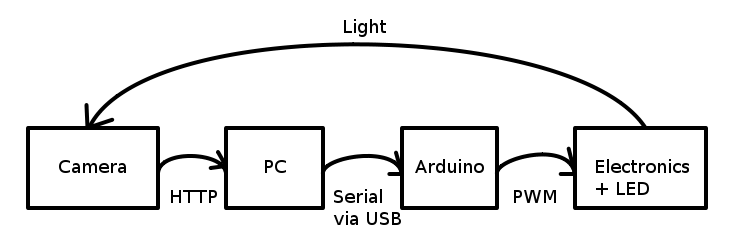
\includegraphics[scale=0.5]{kuvat/commdiagram.png}
 \caption{Systeemin kommunikaatioarkkitehtuuri}
 \label{fig:kommunikaatio}
 \end{center}
\end{figure}

PC lukee kuvan histogrammi-informaation kameralta käyttäen Ethernet-yhteyttä, suorittaa säätöalgoritmin ja antaa ohjauskäskyn (haluttu pulssisuhde) Arduinolle USB-portin kautta. Arduino muuttaa ohjauskäskyn pulssinleveysmodulaatiosignaaliksi ja analogiaelektroniikka vahvistaa sen LED-valaisimen vaatimalle tasolle.

Todellinen systeemi näkyy kuvassa \ref{fig:systeemi}.

\begin{figure}[htcb]
 \begin{center}
  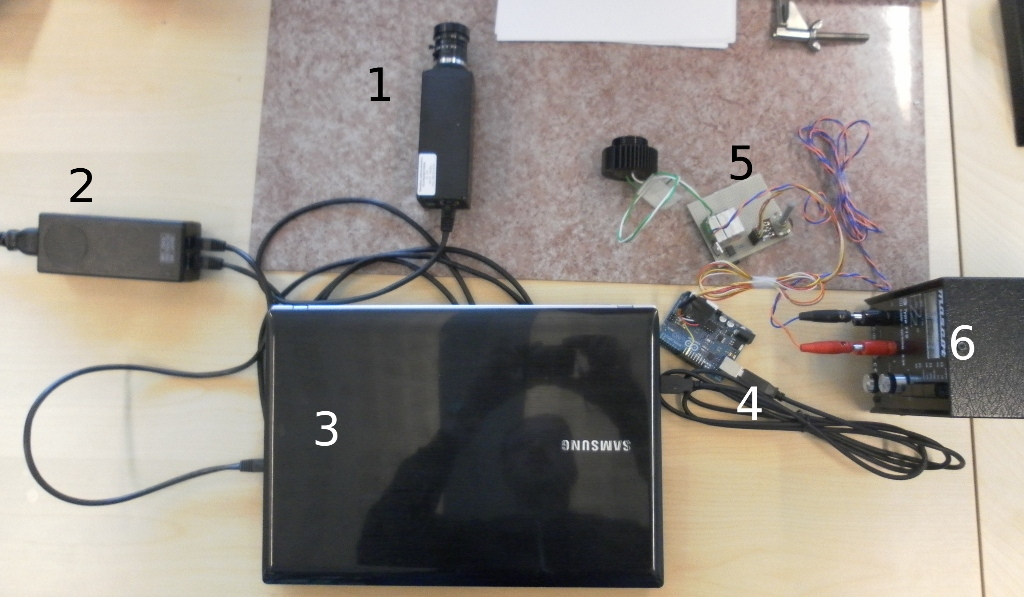
\includegraphics[scale=0.4]{kuvat/systeemi.jpg}
  \caption{Todellinen systeemi. Kuvassa: 1. kamera, 2. kameran teholähde, 3. PC, 4. Arduino Uno, 5. custom-elektroniikka, 6. 12V jännitelähde.}
  \label{fig:systeemi}
 \end{center}

\end{figure}


\subsection{Kamera}

Kamerana on käytetty Elphelin mallia 353 \cite{Elphel}. Se on sekä raudaltaan että ohjelmistoltaan avoin, mikä helpottaa erilaisten custom-sovellusten tekoa. Se pitää sisällään FPGA:n, joka pyörittää minimalistista web-palvelinta PHP-tuella. Tätä käytettiin hyväksi ja palvelimelle kirjoitettiin PHP-ohjelma, joka pyydettäessä hakee kameran muistista senhetkisen komposiittihistogrammidatan ja tarjoilee sen välilyönnein erotettuina desimaalikoodattuina arvoina. 

\subsection{Arduino Uno}

Arduino \cite{Arduino} on avoimen arkkitehtuurin projekti, jonka referenssituote Uno on. Se on tarkoitettu prototyyppialustaksi, johon se onkin omiaan: kehitystyö on nopeaa ja vaivatonta, koska piirilevyltä ja ohjelmistosta löytyy valmiina tuki suurimmalle osalle usein tarvittavista ominaisuuksista, kuten sarjamuotoiselle kommunikaatiolle USB:n yli sekä digitaalisten ja analogisten sisään- ja ulostulojen monipuoliseen hallitsemiseen. Arduinon voi myös ohjelmoida vaivattomasti USB:n kautta. Tässä projektissa piiriä käytetään vain USB:n yli kommunikoitavan PWM-pulssisuhdearvon muuttamiseen PWM-signaaliksi.

Arduino-piiri saa käyttöjännitteensä USB-liitännästä. Seuraavia I/O- ja muita pinnejä on käytetty:

\begin{itemize}
 \item \textit{Digital Pin 9}: PWM-signaali analogiaelektroniikalle
 \item \textit{Digital Pin 8}: jos tämä pinni on kytkettynä GND-pinniin, piiri toimii manuaalimoodissa; jos ei, on automaattinen moodi valittuna.
 \item \textit{Analog In 3}: manuaalimoodin input-signaali potentiometriltä
 \item \textit{5V}: 5 voltin käyttöjännite manuaalimoodin potentiometrille
 \item \textit{GND}: maataso sekä PWM:ää että potentiometriä varten
\end{itemize}

\begin{figure}[htcb]
 \begin{center}
  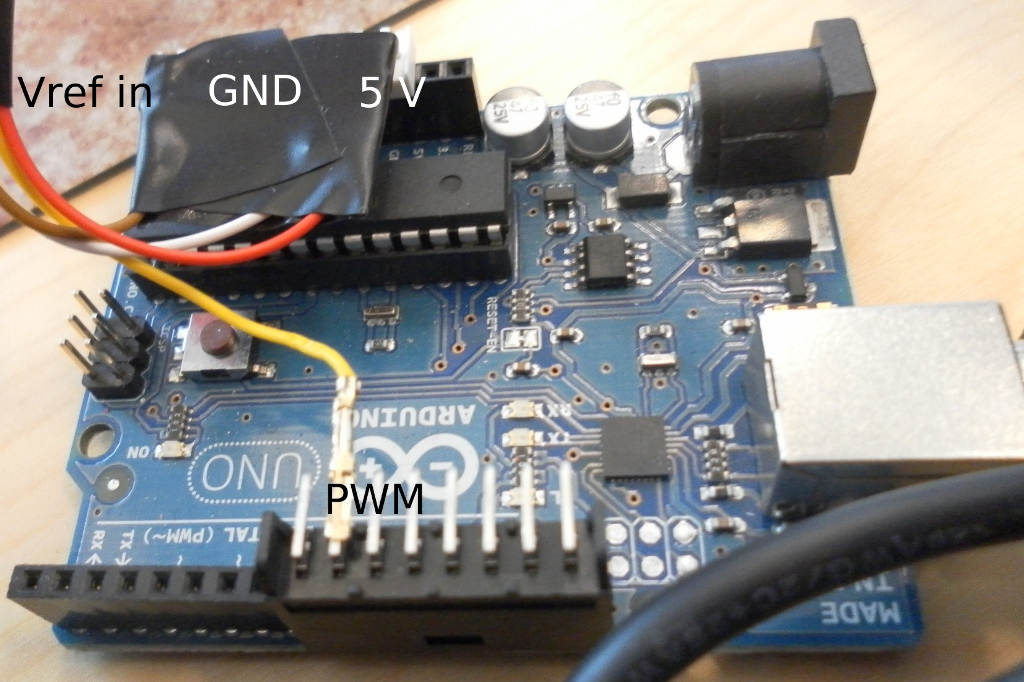
\includegraphics[scale=0.4]{kuvat/arduino.jpg}
  \caption{Arduino Uno liittimet kytkettyinä.}
  \label{fig:arduino}
 \end{center}

\end{figure}



\subsection{Analogiaelektroniikka}

Kuvassa \ref{fig:schema} näkyy rakennetun elektroniikan kytkentäkaavio ja kuvassa \ref{fig:piiri} itse piirilevy. Piirin tarkoitus on vahvistaa Arduinolta tuleva PWM-signaali niin, että IR-LEDin voi liittää suoraan piiriin ilman mitään ylimääräisiä kytkentöjä. Tätä varten piiriltä löytyy myös 5 ohmin tehoetuvastus LEDin virran rajoittamiseksi.

\begin{figure}[htcb]
 \begin{center}
 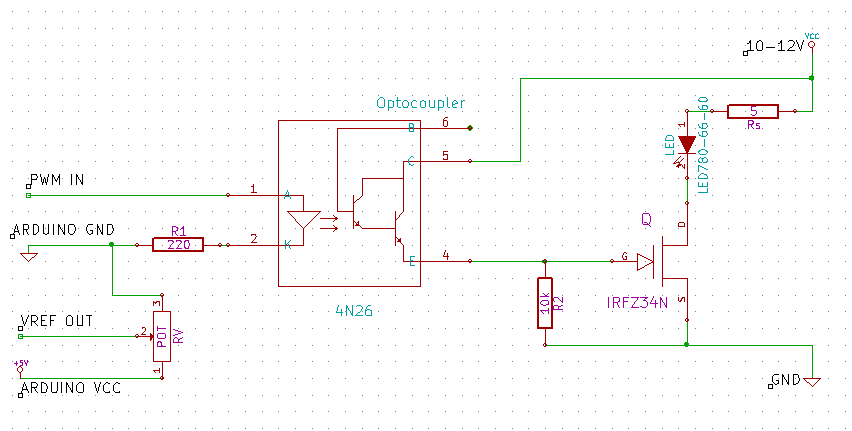
\includegraphics[scale=0.5]{kuvat/schema.png}
 \caption{Projektia varten toteutetun analogiapiirin kytkentäkaavio}
 \label{fig:schema}
 \end{center}
\end{figure}

\begin{figure}[htcb]
 \begin{center}
 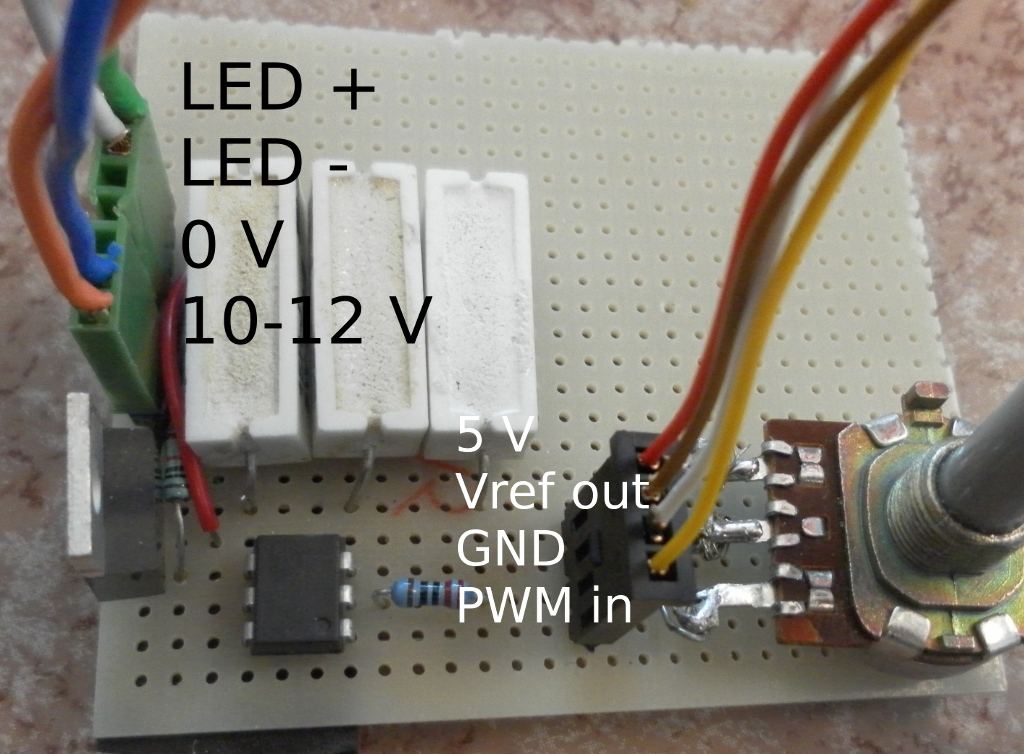
\includegraphics[scale=0.25]{kuvat/piiri_liittimet.jpg}
 \caption{Projektia varten toteutettu analogiapiiri ja sen liitännät}
 \label{fig:piiri}
 \end{center}
\end{figure}

Arduino on optisesti erotettu korkeamman käyttöjännitteen piiristä. Käytetyn IR-LEDin nimellinen jännitehäviö on 9 V ja maksimivirta 600 mA. Etuvastus on mitoitettu niin, että LEDin maksimivirta saavutetaan 12 V käyttöjännitteellä, jolloin vastuksen nimellisen tehonkeston varmuusvara on vielä yli kahdeksankertainen. Haluttua maksimivirtaa voi siis säätää tietyissä rajoissa käyttöjännitettä muuttamalla, mutta toki myös maksimipulssisuhdetta ohjelmallisesti rajoittamalla. Piiri on pyritty suunnittelemaan niin, että mahdollisissa kaapelien oikosulkutapauksissakin LEDin virta on aina vastusten rajoittamaa. Toisin sanoen kumpikaan LEDin johtimista ei ole suoraan käyttöjännitteessä tai maassa kiinni.

Piirissä käytetty kytkinelementti on hyvin alhaisen johtavan moodin jännitehäviön omaava HEXFET (\textit{IRFZ34N}). Nimellisesti se kestää 40 ampeerin virran, mutta se tuskin tulee tarpeeseen. Alhaisesta jännitehäviöstä ja kytkintoiminnallisuudesta johtuen FET ei tarvitse jäähdytinelementtiä, mutta se on joka tapauksessa sijoitettu piirin reunalle jäähdytyksen mahdollistamiseksi.

Piirissä on myös yksi potentiometri, jolla voi manuaalisesti säätää Arduinon tarjoaman PWM-signaalin pulssisuhdetta. Tämä tehtiin lähinnä debug- ja mittaustarkoituksiin.

12 voltin käyttöjännitteellä piirin hyötysuhde (LEDin kuluttama teho jaettuna kokonaisteholla) on n. 75\%; hukkatehosta suurin osa (1,8 W maksimipulssisuhteella) muuttuu lämmöksi etuvastuksessa.

\subsection{PC}

\subsubsection{Liitännät}

PC keskustelee kameran kanssa Ethernetin välityksellä. Kamera kytketään suoraan PC:n Ethernet-porttiin ja tietokoneen IP-asetukset on konfiguroitava sisäverkkoalueelle 192.168.0.xxx. Kameran IP on oletuksena 192.168.0.9. Kameraa pystyy käyttämään ja manipuloimaan sekä sen HTTP-serverin että suoran SSH- tai TELNET-yhteyden kautta. Kameran sisäisen FPGA:n käyttöjärjestelmänä on riisuttu Linux.

Arduinon kanssa puolestaan keskustellaan virtuaalisen sarjaportin kautta. Fyysisesti Arduino liitetään USB-porttiin, ja tunnistettuaan laitteen PC luo sitä vastaavan virtuaalisen COM-portin. Käyttöä varten on tunnistettava kyseinen portti ja tallennettava sen tunniste konfiguraatiotiedostoon. Tämä toimii sekä Windows- että Linux-alustalla, mutta portin tunniste vaihtelee alustasta riippuen.

\subsubsection{Ohjelman alusta ja rakenne}

Säätöön tarkoitettu ohjelma on tehty Pythonilla ja sitä on ajettu \textit{Python(x,y)} -sovelluksella Windows-ympäristössä. Käyttöjärjestelmällä tai virtuaalikoneella ei ole merkitystä, mutta \textit{pySerial}-moduuli tulee olla asennettuna sarjaliikennettä varten. Ohjelma on säikeistetty ja jokseenkin modulaarinen; olio-ohjelmointia on hyödynnetty.

Ohjelma koostuu pääohjelmasta ja muutamasta lisämoduulista. Jako on seuraavanlainen:

\begin{itemize}
 \item \textit{control.py}: main-funktio, muutama apufunktio mm. konfiguraation parsimiseen sekä säikeistetty Controller-luokka, joka on vastuussa itse säädöstä.
 \item \textit{SerialInputMonitor.py}: moduuli sisääntulevan sarjaliikenteen monitorointiin. Säikeistetty.
 \item \textit{HistogramMonitor.py}: moduuli histogrammidatan visualisoimiseen. Ei käytetä, koska kameran ``Advanced Webcam'' -sovellus sopii paremmin tarkoitukseen.
 \item \textit{config.conf}: sisältää mm. kameran IP-osoitteen, käytetyn COM-portin tunnisteen sekä muita konfiguraatioparametreja.
\end{itemize}

\subsubsection{Säätöalgoritmi}

Säätöalgoritmi on PID-johdannainen ja perustuu kameralta saatavaan histogrammidataan. Olennaista on välttää informaation hukkaaminen, joten ylivalottumisen esto on prioriteettilistassa korkeimpana - siispä suurimman painokertoimen virhetermiä muodostettaessa saa histogrammin yläpään painotettu keskiarvo. Toisena prioriteettina on alivalottumisen esto, ja kolmantena histogrammin painopisteen säätäminen haluttuun kohtaan (tällä hetkellä kirkkausarvo 172). Säätöalgoritmin voi esittää kaavana:

\begin{equation}
 e_n = a \cdot \sum_{i=240}^{255} (i - 239) \cdot h_{n,i} + b \cdot \sum_{i=0}^{10} (11-i) \cdot h_{n,i} + c \cdot (L - \frac{\sum_{i=0}^{255}i \cdot h_{n,i}}{\sum_{i=0}^{255}h_n,i})
\end{equation}
\begin{equation}
 s_n = s_{n-1} + P \cdot e_n + D \cdot \frac{de}{dt} ,
\end{equation}

jossa $e_n$ on virhetermin arvo hetkellä \textit{n}, $h_{n,i}$ on histogrammin alkion \textit{i} arvo ajanhetkellä \textit{n}, $a, b, c, P, D$ painokertoimia, \textit{L} haluttu histogrammin painopiste ja $s_n$ ohjauksen (eli halutun pulssisuhteen) arvo hetkellä \textit{n}.

Lyhyesti tiivistettynä ohjausarvoa siirretään joka iteraatio havaittua virhettä korjaavaan suuntaan. Aika-askel on 250 millisekuntia. Kameran ominaisuudet sallisivat suuremmankin säätötaajuuden, mutta sitä ei nähty tarpeelliseksi.

\section{Työn eteneminen}

Työ päästiin aloittamaan kunnolla vasta huhtikuun puolella, kun kaikki laitteet saatiin paikalle. Tätä ennen oli saatu tehtyä arduino-kommunikaatio ja myös runko pääohjelmalle sekä tutustuttu kirjallisuuteen. Heti laitteiden saapumisen jälkeen n. yksi työpäivä käytettiin kameran liittämiseen PC:een ja sen ominaisuuksien tutkimiseen. Todettiin, että jo lähes valmiiksi tehtyä histogrammimonitoria ei tarvitakaan toiminnan visualisoimiseksi, koska kamerassa löytyy valmiina \textit{Advanced Webcam} -sovellus, joka näyttää myös histogrammidatan kuvan ohessa.

Yleisesti ottaen lähes kaikkia projektin osa-alueita kehitettiin enemmän tai vähemmän rinnakkain. Ainoastaan Arduinon koodi saatiin lopputilaansa aikaisin, jo maaliskuussa. Työ oli itsenäistä, osittain koska ohjaaja oli harvoin paikalla mutta myös koska projektin suuntaviivat olivat alusta asti selvät eikä erityisiä ongelmia esiintynyt.

Kokonaisuudessaan, hieman yllättäenkin, suurin osa käytetystä ajasta kului elektroniikan rakentamiseen, vaikka varsinaisia iteraatiokierroksia ei suunnittelussa esiintynytkään. Myös yleiseen testaukseen ja parametrien optimointiin kului paljon aikaa. Loppuaika jakautui melko tasan eri laitteiden välisen kommunikaation toteuttamiseen, ohjelmointiin ja itse säätöalgoritmin toteuttamiseen. Arvioitu tuntitilanne ennen tämän dokumentin kirjoittamista on esitetty kuvassa \ref{fig:tuntitilanne}. Loppuraportin sekä koodien siistimisen ja kommentoinnin myötä ``dokumentaatio''-kohtaan on lisättävä n. 7h, jolloin yhteistuntimääräksi tulee n. 75h. Kyseessä on arvio tehokkaasta työajasta; toki tunteja kului työhuoneella useampiakin.

\begin{figure}[h]
 \begin{center}
  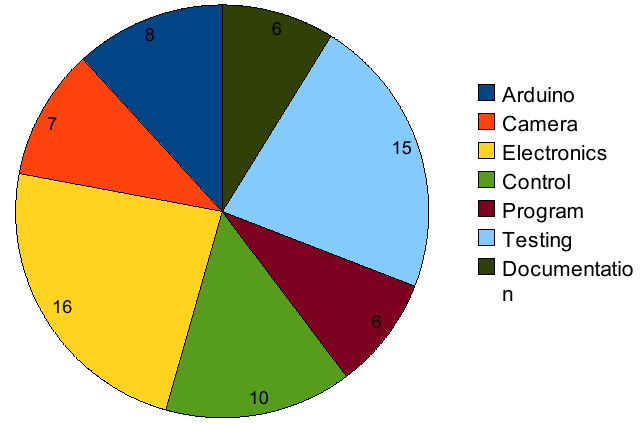
\includegraphics[scale=0.5]{kuvat/tuntitilanne.png}
  \caption{Työtuntijakauma työn eri osa-alueiden kesken. Kaaviosta puuttuu tämän dokumentin tekemiseen sekä koodien siistimiseen ja kommentointiin käytetty aika, 7h.}
  \label{fig:tuntitilanne}
 \end{center}
\end{figure}



\section{Tulokset}

Alkuperäistä käyttötarkoitusta, ICG-kuvantamista varten tarvittavia laitteita (IR-filtterit, varjoaine, koe-eläin tai -henkilö) ei ollut saatavilla, siispä systeemin suorituskykyä mitattiin kuvan \ref{fig:koejarjestely} osoittamalla koejärjestelyllä. Kameran valotus säädettiin sellaiseksi, että LEDin ollessa pois päältä kameran edessä ollut paperi juuri ja juuri näkyi - tämä oletettiin toivotuksi vasteeksi IR-filtteriä käytettäessä. Kameran valotus pidettiin kiinteänä koko kokeen ajan.

\begin{figure}[h]
 \begin{center}
  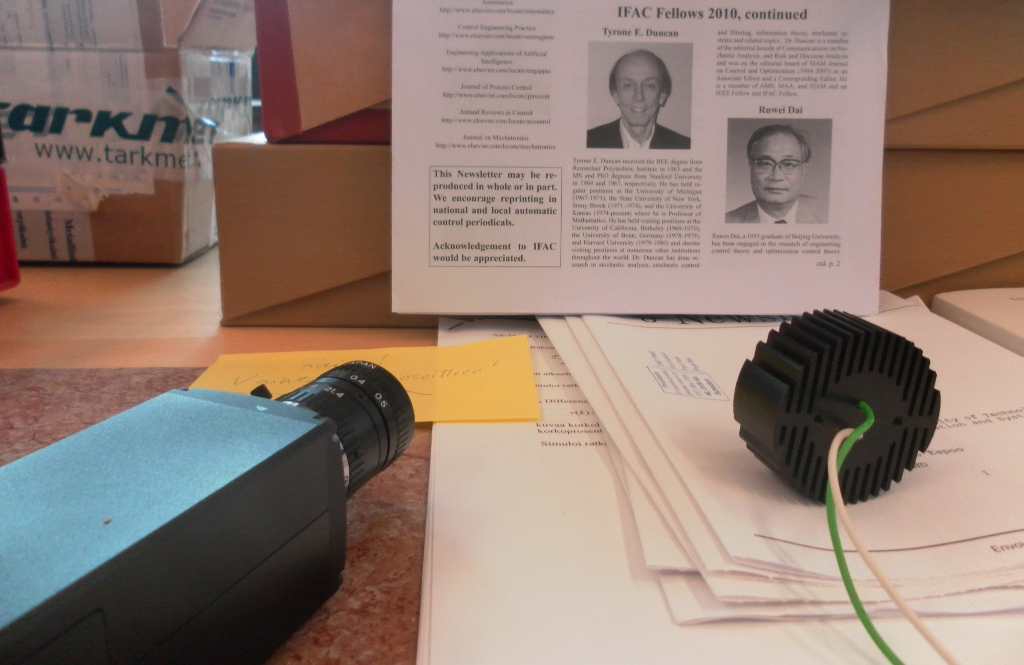
\includegraphics[scale=0.4]{kuvat/koejarjestely.jpg}
  \caption{Koejärjestely - kamera katsoo paperia, jota systeemin ohjaama IR-LED valaisee.}
  \label{fig:koejarjestely}
 \end{center}

\end{figure}


Systeemin käyttäytymistä tutkittiin siirtymällä manuaalimoodista automaattimoodiin sekä ohjausarvosta 0 että 255 (täysi pulssisuhde), ja myös siirtämällä LEDiä lähemmäs tai kauemmas. Systeemin vaste oli nopea ja kaikissa tapauksissa yli- tai alivalotus eliminoitiin nopeasti, 1-4 iteraation kuluessa eli yleensä alle sekunnissa. Vähemmän tärkeä histogrammin painopisteen siirto asettui n. 5 sekunnin kuluessa. Systeemi oli koko testin ajan stabiili, värähtelyjä ei esiintynyt. Kuvassa \ref{fig:tulos} näkyy kamerakuva nolla- ja maksimipulssisuhteella sekä säädön tulos.

\begin{figure}[h]
 \begin{center}
  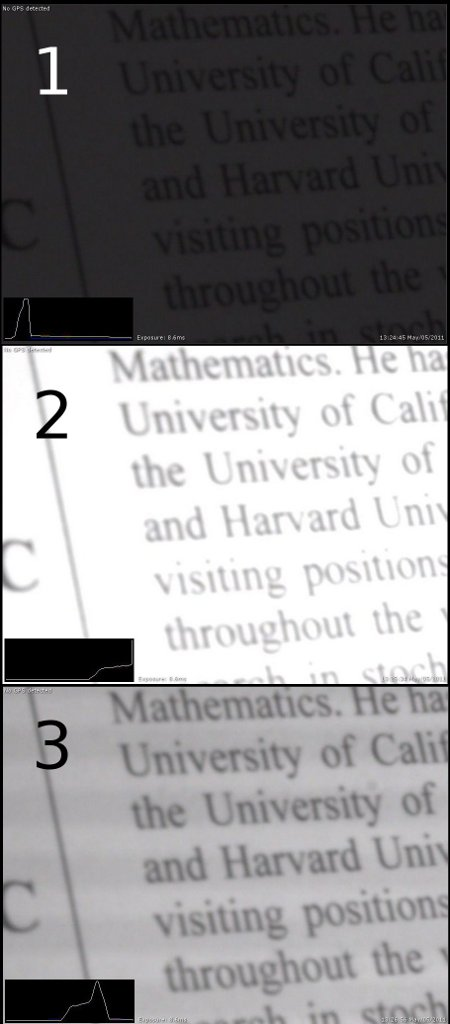
\includegraphics[scale=0.5]{kuvat/tulos.jpg}
  \caption{Suorituskykytestin tulos: systeemi säätää valaistuksen kameralle sopivaksi nopeasti ja tarkasti. Kuva 1: LED pois päältä. Kuva 2: LEDiä ajetaan maksimipulssisuhteella. Kuva 3: LED säädetty optimaaliseksi.}
  \label{fig:tulos}
 \end{center}

\end{figure}


\section{Yhteenveto}

Kehitettiin kamerapohjainen säätöjärjestelmä LED-valaisimelle. Projekti sisälsi kommunikaatio\-rajapintojen luontia ja konfigurointia, säätö\-algoritmin kehitystä ja toteutusta, elektroniikka\-suunnittelua ja -toteutusta sekä yleistä ohjelmointia. Tulokset olivat hyviä, laite toimii vaatimusten mukaisesti. Työhön kului n. 75 tehokasta työtuntia.

Mahdollisia jatkokehityksen kohteita:
\begin{itemize}
 \item Arduinon ja custom-elektroniikan integrointi, kenties kokonaan oman alustan luominen sisältäen elektroniikan, mikrokontrollerin ja RS232/USB-konvertterin
 \item Laitteen kotelointi ja liitinten standardointi
 \item On kenties mahdollista eliminoida PC kokonaan ja ajaa säätöalgoritmia suoraan mikrokontrollerissa. Tämä kuitenkin edellyttää Ethernet-rajapinnan luomista mikrokontrollerille.
\end{itemize}


\clearpage

% liitetaan bibtex-viitteet
\bibliography{asproj-loppuraportti}

\end{document}          
